% Title page and front notes.
\begin{titlepage}
\thispagestyle{empty}
\centering
\vspace*{1.2in}
{\Huge\bfseries Paper Winder\par}
\vspace{0.4em}
{\LARGE Owner's Manual\par}
\vspace{1.5em}
{\Large \machine{} (M1)\par}
\vspace{2.5em}
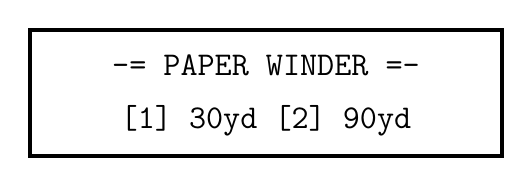
\begin{tikzpicture}
  \draw[line width=1.5pt] (0,0) rectangle (6,1.6);
  \node[font=\ttfamily\large] at (3,1.15) {-= PAPER WINDER =-};
  \node[font=\ttfamily\large] at (3,0.45) {[1] 30yd    [2] 90yd};
\end{tikzpicture}
\par\vspace{2.5em}
{\large Covers firmware version \textbf{fw=\fwver} and the PC program \textbf{winder}\par}
\vspace{0.5em}
{\large Manual revision: \textbf{\revdate}\par}
\vfill
\begin{minipage}{0.85\textwidth}
\small
Keep this manual near the machine. Read Chapter~\ref{ch:safety} (Safety)
before you use the machine for the first time. The quick-reference card in
Appendix~\ref{app:quickref} can be cut out and posted beside the panel.

Support: [SUPPORT CONTACT]\quad Machine serial number: [SERIAL NUMBER]
\end{minipage}
\end{titlepage}
